%!TEX program = xelatex
% 完整编译: xelatex -> biber/bibtex -> xelatex -> xelatex
\documentclass[lang=cn,a4paper,newtx]{elegantpaper}

\newcommand{\dmodel}{d_{\text{model}}}
\newcommand{\dff}{d_{\text{ff}}}

\title{注意力机制就是你所需要的一切}
\author{左元翻译}

% 本文档命令
\usepackage{array}
\newcommand{\ccr}[1]{\makecell{{\color{#1}\rule{1cm}{1cm}}}}

\newcommand{\dsri}{DeepSeek-R1}
\newcommand{\dsro}{DeepSeek-R1-Zero}

\begin{document}

\maketitle

\begin{abstract}
  主流的序列转换模型基于复杂的循环神经网络(RNN)或卷积神经网络(CNN),这些模型通常包含编码器和解码器。表现最佳的模型还通过注意力机制连接编码器和解码器。我们提出了一种新的简单网络架构——Transformer,它完全基于注意力机制,彻底摒弃了循环和卷积结构。在两个机器翻译任务上的实验表明,这些模型在质量上更优,同时具有更高的并行性,并且训练所需的时间显著减少。我们的模型在WMT 2014英语到德语翻译任务中取得了28.4的BLEU分数,比现有的最佳结果(包括集成模型)提高了超过2个BLEU分数。在WMT 2014英语到法语翻译任务中,我们的模型在8个GPU上训练了3.5天后,取得了41.8的BLEU分数,创下了单一模型的最新记录,而训练成本仅为文献中最佳模型的一小部分。我们通过将Transformer成功应用于英语句法解析任务(无论是大规模还是有限训练数据)表明,Transformer能够很好地推广到其他任务中。
\end{abstract}

\newpage

\tableofcontents

\newpage

\section{简介}

循环神经网络(RNN),特别是长短期记忆网络(LSTM)和门控循环神经网络(GRU),已被牢固确立为序列建模和转换问题(如语言建模和机器翻译)中的最先进方法。此后,众多研究不断推动循环语言模型和编码器-解码器架构的边界。

循环模型通常沿着输入和输出序列的符号位置进行因式分解计算。将位置与计算时间的步骤对齐,它们会生成一系列隐藏状态 $h_t$(作为前一个隐藏状态 $h_{t-1}$ 和位置 $t$ 的输入的函数)。这种固有的顺序性质阻碍了训练示例内的并行化,这在序列长度较长时变得尤为关键,因为内存限制会限制跨示例的批处理。最近的研究通过因式分解技巧和条件计算在计算效率方面取得了显著改进,同时在后一种情况下也提高了模型性能。然而,顺序计算的基本约束仍然存在。

注意力机制已经成为各种任务中引人注目的序列建模和转换模型的一个组成部分,它允许对依赖关系进行建模,而无需考虑它们在输入或输出序列中的距离。然而,在几乎所有情况下,这种注意力机制都是与循环网络结合使用的。

在这项工作中,我们提出了Transformer,这是一种摒弃了循环结构、完全依赖注意力机制来捕捉输入与输出之间全局依赖关系的模型架构。Transformer能够实现显著更高的并行化,并且在仅使用8个P100 GPU训练12小时后,就能在翻译质量上达到新的最先进水平。

\section{背景}

减少顺序计算的目标也构成了扩展神经GPU(Extended Neural GPU)、ByteNet和ConvS2S的基础,所有这些模型都使用卷积神经网络作为基本构建块,并行计算所有输入和输出位置的隐藏表示。在这些模型中,关联两个任意输入或输出位置的信号所需的运算数量随着位置之间的距离而增加,对于ConvS2S是线性增长,对于ByteNet是对数增长。这使得学习远距离位置之间的依赖关系变得更加困难。在Transformer中,这一运算数量被减少到了常数级别。虽然对注意力加权位置进行平均而导致了有效分辨率降低,但我们通过多头注意力机制(如第\ref{sec:attention}节所述)抵消了这一影响。

自注意力机制,有时也称为内部注意力机制,是一种将单个序列的不同位置关联起来以计算序列表示的注意力机制。自注意力机制已成功应用于各种任务,包括阅读理解、文本摘要、文本蕴含和学习任务无关的句子表示。

端到端记忆网络基于循环注意力机制,而不是序列对齐的循环结构,并且已被证明在简单语言问答和语言建模任务中表现良好。

然而,据我们所知,Transformer是第一个没有使用序列对齐的RNN或卷积,而完全依赖自注意力机制来计算其输入和输出表示的转换模型。在接下来的章节中,我们将描述Transformer,解释自注意力机制,并讨论其相对于《Neural GPUs learn algorithms》、《Neural machine translation in linear time》和《Convolutional sequence to sequence learning》等模型的优势。

\section{模型架构}

\begin{figure}
  \centering
  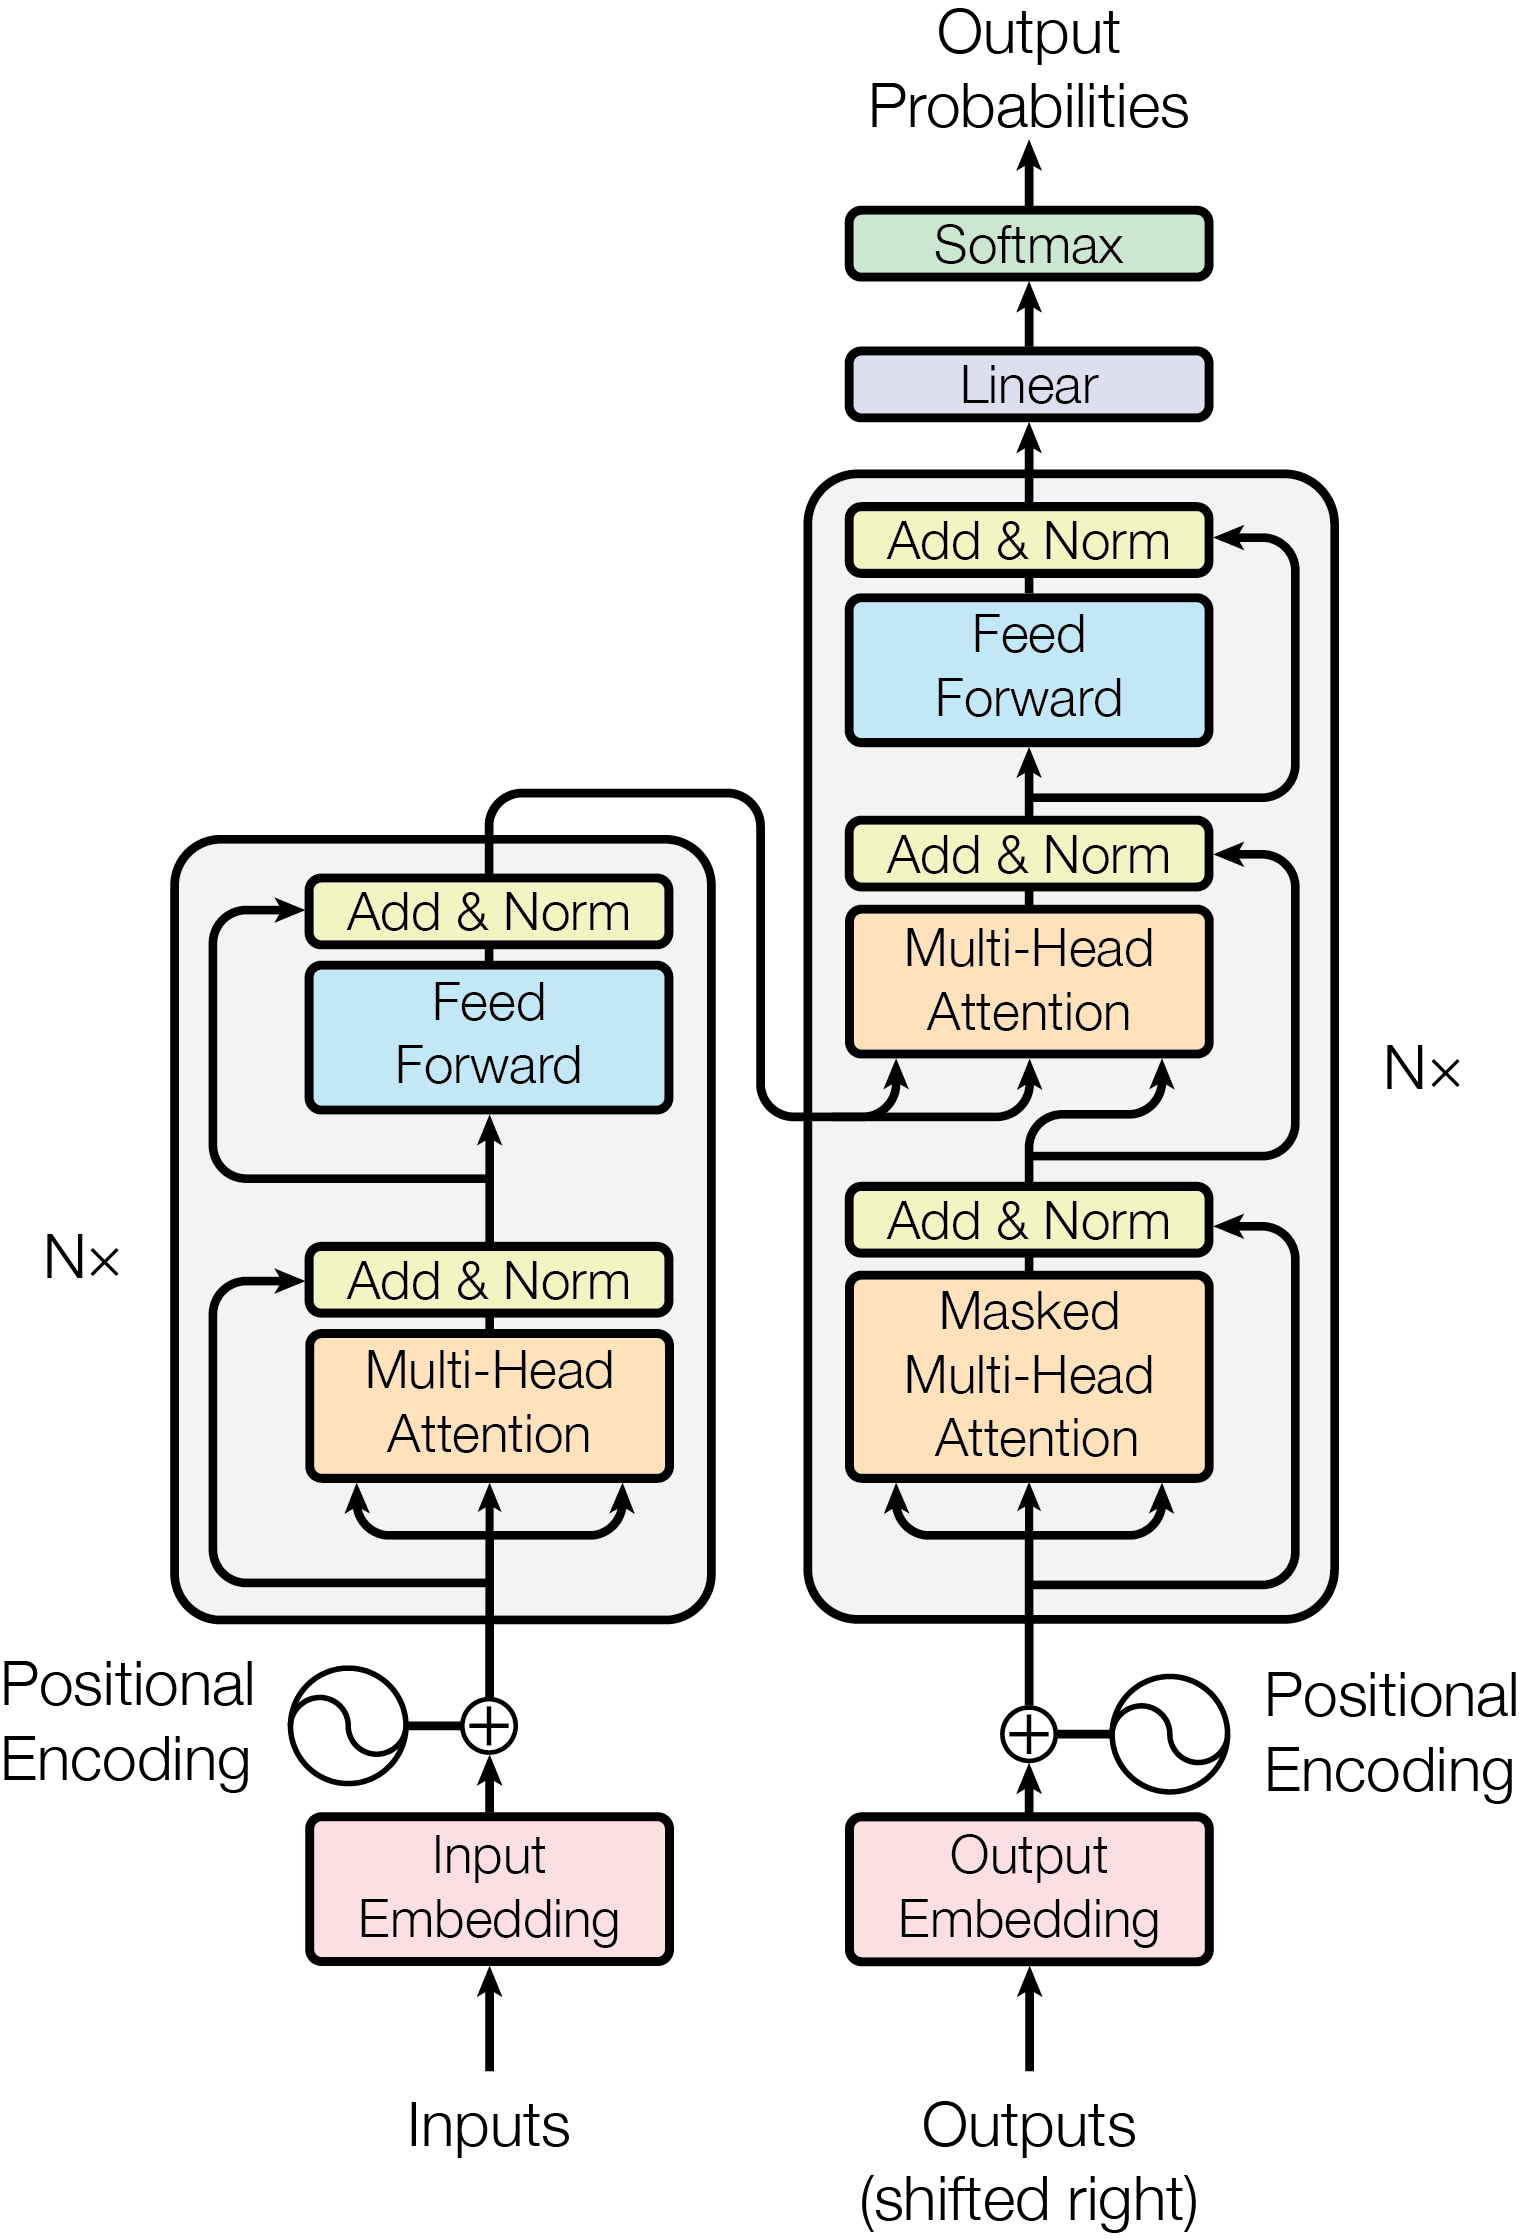
\includegraphics[scale=0.6]{Figures/ModalNet-21}
  \caption{Transformer模型架构。}
  \label{fig:model-arch}
\end{figure}

大多数具有竞争力的神经序列转换模型都采用编码器-解码器结构。在这里,编码器将输入符号表示序列 $(x_1, ..., x_n)$ 映射为连续表示序列 $\mathbf{z} = (z_1, ..., z_n)$。给定 $\mathbf{z}$,解码器随后逐个元素地生成符号输出序列 $(y_1,...,y_m)$。在每一步中,模型都是自回归的,在生成下一个符号时,将之前生成的符号作为额外输入。

Transformer遵循这种整体架构,在编码器和解码器中均使用堆叠的自注意力机制和逐点全连接层,分别如图~\ref{fig:model-arch}的左右两部分所示。

\subsection{编码器和解码器的堆叠}

\paragraph{编码器:}编码器由$N=6$个相同的层堆叠而成。每一层包含两个子层。第一个子层是多头自注意力机制,第二个子层是一个简单的逐点全连接前馈网络。我们在每个子层周围采用了残差连接,随后进行层归一化。也就是说,每个子层的输出为$\mathrm{LayerNorm}(x + \mathrm{Sublayer}(x))$,其中$\mathrm{Sublayer}(x)$是该子层自身实现的函数。为了便于这些残差连接,模型中的所有子层以及嵌入层的输出维度均为$\dmodel=512$。

\paragraph{解码器:}解码器同样由$N=6$个相同的层堆叠而成。除了每个编码器层中的两个子层外,解码器还插入了第三个子层,该子层对堆叠的编码器的输出执行多头注意力机制。与编码器类似,我们在每个子层周围采用了残差连接,随后进行层归一化。我们还修改了堆叠的解码器中的自注意力子层,以防止位置关注到后续位置。这种掩码机制,结合输出嵌入偏移一个位置的事实,确保了对位置$i$的预测只能依赖于位置小于$i$的已知输出。

\subsection{注意力机制} \label{sec:attention}

注意力函数可以描述为将查询和一组键值对映射到输出,其中查询、键、值和输出都是向量。输出计算为值的加权和,其中分配给每个值的权重通过查询与相应键的兼容性函数计算得出。

\subsubsection{缩放点积注意力(Scaled Dot-Product Attention)} \label{sec:scaled-dot-prod}

我们将这个特定的注意力机制称为“缩放点积注意力”(图~\ref{fig:multi-head-att})。输入包括维度为$d_k$的查询和键,以及维度为$d_v$的值。我们计算查询与所有键的点积,将每个点积除以$\sqrt{d_k}$,然后应用softmax函数以获得值的权重。

在实际运算中,我们同时计算一组查询的注意力函数,这些查询被打包成一个矩阵$Q$。键和值也被打包成矩阵$K$和$V$。我们计算输出矩阵如下:

\begin{equation}
  \mathrm{Attention}(Q, K, V) = \mathrm{softmax}(\frac{QK^T}{\sqrt{d_k}})V
\end{equation}

两种最常用的注意力函数是加性注意力和点积(乘性)注意力。点积注意力与我们的算法相同,只是没有$\frac{1}{\sqrt{d_k}}$的缩放因子。加性注意力使用具有单个隐藏层的前馈网络来计算兼容性函数。尽管两者在理论复杂度上相似,但在实践中,点积注意力速度更快且空间效率更高,因为它可以使用高度优化的矩阵乘法代码来实现。

虽然对于较小的$d_k$值,两种机制表现相似,但对于较大的$d_k$值,加性注意力在未缩放的情况下优于点积注意力。我们推测,对于较大的$d_k$值,点积的幅度会变得很大,从而将softmax函数推向梯度极小的区域\footnote{为了说明为什么点积会变大,假设$q$和$k$的分量是均值为$0$、方差为$1$的独立随机变量。那么它们的点积$q \cdot k = \sum_{i=1}^{d_k} q_ik_i$的均值为$0$,方差为$d_k$。}。为了抵消这种影响,我们将点积缩放$\frac{1}{\sqrt{d_k}}$。

\subsubsection{多头注意力机制(Multi-Head Attention)} \label{sec:multihead}

\begin{figure}
\begin{minipage}[t]{0.5\textwidth}
  \centering
  缩放点乘注意力机制 \\
  \vspace{0.5cm}
  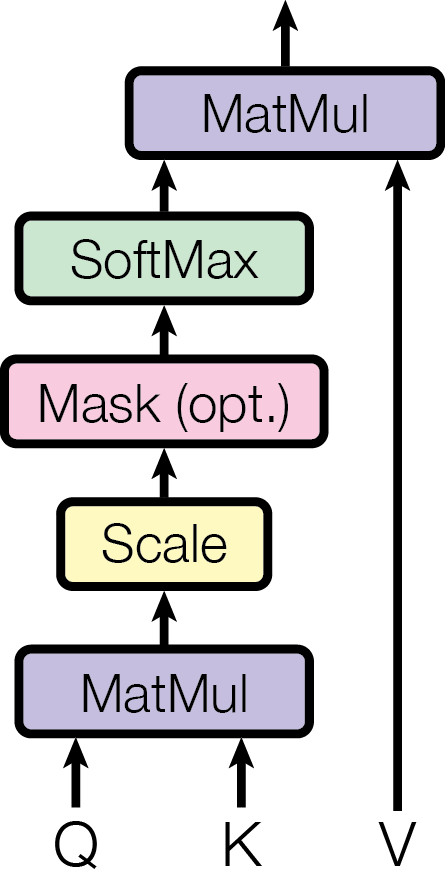
\includegraphics[scale=0.6]{Figures/ModalNet-19}
\end{minipage}
\begin{minipage}[t]{0.5\textwidth}
  \centering 
  多头注意力机制 \\
  \vspace{0.1cm}
  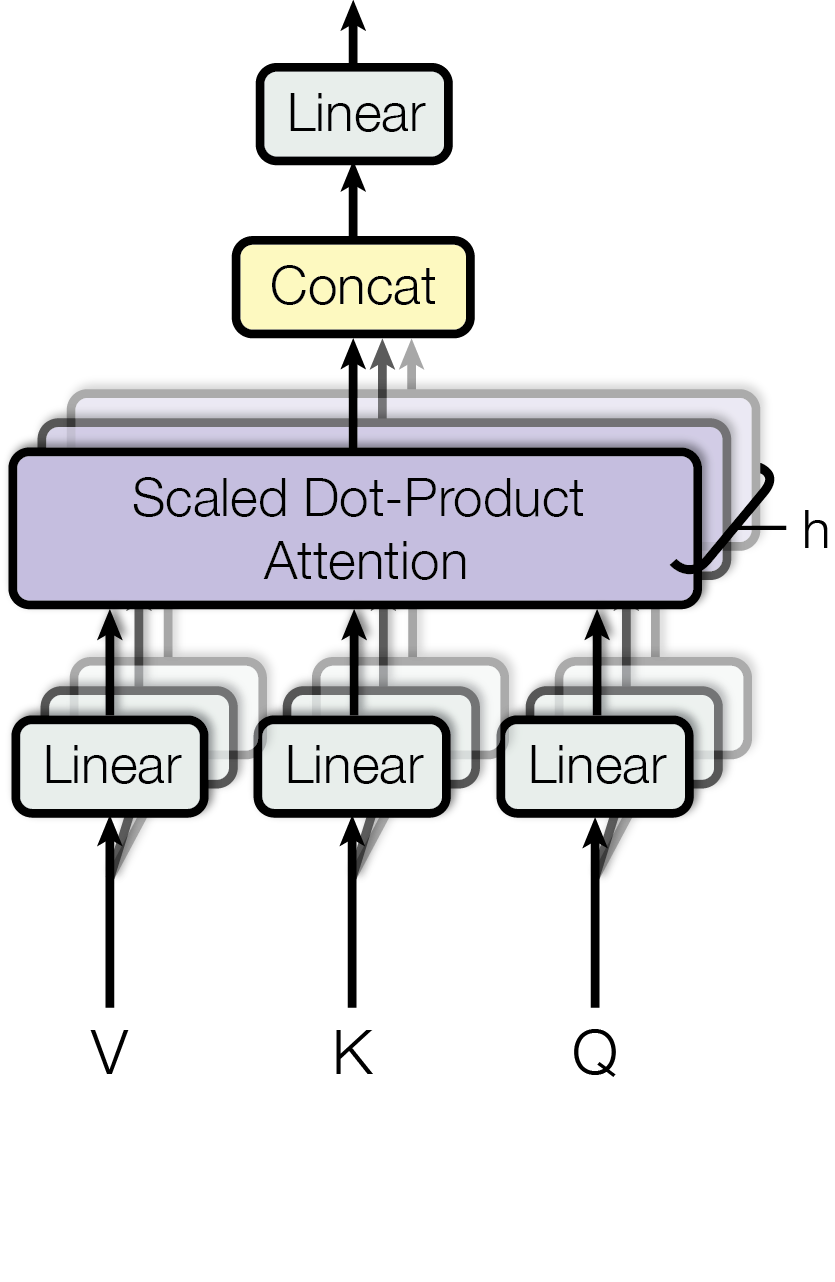
\includegraphics[scale=0.6]{Figures/ModalNet-20}  
\end{minipage}


  % \centering

  \caption{(左) 缩放点乘注意力机制。(右) 包含多个并行的注意力层的多头注意力机制。}
  \label{fig:multi-head-att}
\end{figure}

我们发现,与其使用$\dmodel$维的键、值和查询执行单一的注意力函数,不如将查询、键和值(分别通过不同的、可学习的线性投影)线性投影$h$次到$d_k$、$d_k$和$d_v$维度更为有益。在这些投影后的查询、键和值版本上,我们并行地执行注意力函数,得到$d_v$维的输出值。这些输出值被连接起来并再次投影,最终得到结果值,如图~\ref{fig:multi-head-att}所示。

多头注意力机制允许模型同时关注来自不同位置的不同表示子空间的信息。在单一注意力头的情况下,平均化会抑制这种能力。

\begin{align*}
  \mathrm{MultiHead}(Q, K, V) &= \mathrm{Concat}(\mathrm{head_1}, ..., \mathrm{head_h})W^O\\
  \text{where}~\mathrm{head_i} &= \mathrm{Attention}(QW^Q_i, KW^K_i, VW^V_i)\\
\end{align*}

其中投影是可学习的参数矩阵,分别为 $W^Q_i \in \mathbb{R}^{\dmodel \times d_k}$、$W^K_i \in \mathbb{R}^{\dmodel \times d_k}$、$W^V_i \in \mathbb{R}^{\dmodel \times d_v}$ 和 $W^O \in \mathbb{R}^{hd_v \times \dmodel}$。

在这项工作中,我们采用了$h=8$个并行的注意力层,即注意力头。对于每个注意力头,我们使用$d_k=d_v=\dmodel/h=64$。由于每个头的维度降低,总计算成本与全维度的单头注意力相似。

\subsubsection{注意力机制在我们模型中的应用}

Transformer 在三种不同的场景中使用多头注意力机制:

\begin{itemize}
 \item 在“编码器-解码器注意力”层中,查询来自解码器的前一层的输出,而记忆键和值则来自编码器的输出。这使得解码器中的每个位置都可以关注输入序列中的所有位置。这模仿了序列到序列模型中典型的编码器-解码器注意力机制。

 \item 编码器包含自注意力层。在自注意力层中,所有的键、值和查询都来自同一个地方,即编码器前一层的输出。编码器中的每个位置可以关注编码器前一层的所有位置。

 \item 类似地,解码器中的自注意力层允许解码器中的每个位置关注解码器中包括该位置在内的所有位置。为了保持自回归特性,需要防止解码器中的信息向左流动,所以我们在缩放点积注意力中通过屏蔽(设置为$-\infty$)softmax输入中所有对应非法连接的值来实现这一点。参见图~\ref{fig:multi-head-att}。

\end{itemize}

\subsection{逐位置前馈网络(Position-wise Feed-Forward Networks)}\label{sec:ffn}

除了注意力子层外,我们的编码器和解码器的每一层还包含一个全连接的前馈网络,该网络分别且相同地应用于每个位置。它由两个线性变换组成,中间通过ReLU激活函数连接。

\begin{equation}
  \mathrm{FFN}(x)=\max(0, xW_1 + b_1) W_2 + b_2
\end{equation}

尽管线性变换在不同位置上是相同的,但它们在每一层中使用不同的参数。另一种描述方式是将其视为两个核大小为1的卷积。输入和输出的维度为$\dmodel=512$,而内层的维度为$d_{ff}=2048$。

\subsection{嵌入和Softmax}

与其它序列转换模型类似,我们使用可学习的嵌入将输入tokens和输出tokens转换为维度为$\dmodel$的向量。我们还使用常见的可学习线性变换和softmax函数将解码器输出转换为预测的下一个token的概率。在我们的模型中,我们在两个嵌入层和softmax前的线性变换之间共享相同的权重矩阵,类似于。在嵌入层中,我们将这些权重乘以$\sqrt{\dmodel}$。

\subsection{位置编码(Positional Encoding)}

由于我们的模型不包含循环和卷积结构,为了让模型能够利用序列的顺序信息,我们必须注入一些关于序列中token的相对或绝对位置的信息。为此,我们在堆叠的编码器和解码器的底部向输入嵌入中添加了“位置编码”。位置编码的维度$\dmodel$与嵌入的维度相同,因此两者可以相加。位置编码有多种选择,包括可学习的位置编码和固定的位置编码。

在这项工作中,我们使用了不同频率的正弦和余弦函数:

\begin{align*}
  PE_{(pos,2i)} = sin(pos / 10000^{2i/\dmodel}) \\
  PE_{(pos,2i+1)} = cos(pos / 10000^{2i/\dmodel})
\end{align*}

其中$pos$表示位置,$i$表示维度。也就是说,位置编码的每个维度对应于一个正弦曲线。波长从$2\pi$到$10000 \cdot 2\pi$形成一个几何级数。我们选择这个函数是因为我们假设它可以让模型更容易地学习通过相对位置进行关注,因为对于任何固定的偏移量$k$,$PE_{pos+k}$可以表示为$PE_{pos}$的线性函数。

我们还尝试了使用可学习的位置嵌入,发现这两种方法产生的结果几乎相同(见表~\ref{tab:variations} 行 (E))。我们选择了正弦版本,因为它可能使模型能够外推到比训练期间遇到的更长的序列长度。

\section{为什么使用自注意力机制?}

在本节中,我们将自注意力层的各个方面与常用于将一个变长符号表示序列$(x_1, ..., x_n)$映射到另一个等长序列$(z_1, ..., z_n)$的循环层和卷积层进行比较,其中$x_i, z_i \in \mathbb{R}^d$,例如典型序列转换编码器或解码器中的隐藏层。为了说明我们使用自注意力机制的动机,我们考虑了三个需求。

其一是每层的总计算复杂度。其二是可以并行化的计算量,以所需的最小顺序运算数来衡量。

其三是网络中长距离依赖之间的路径长度。学习长距离依赖是许多序列转换任务中的一个关键挑战。影响学习这种依赖能力的一个关键因素是前向和反向信号在网络中必须遍历的路径长度。输入和输出序列中任意位置组合之间的路径越短,学习长距离依赖就越容易。因此,我们还比较了由不同类型层组成的网络中任意两个输入和输出位置之间的最大路径长度。

\begin{table}[t]
\caption{
  不同层类型的最大路径长度,每层的复杂度和顺序运算的最小数量。 $n$ 是序列长度,$d$ 是表示的维度,$k$ 是卷积的核大小,$r$ 是受限的自注意力机制的邻域的大小。}
\label{tab:op_complexities}
\begin{center}
\vspace{-1mm}

\begin{tabular}{lccc}
\toprule
层的类型   & 每层的复杂度 & 顺序 & 最大路径长度  \\
           &             & 运算 &   \\
\hline
\rule{0pt}{2.0ex}Self-Attention & $O(n^2 \cdot d)$ & $O(1)$ & $O(1)$ \\
Recurrent & $O(n \cdot d^2)$ & $O(n)$ & $O(n)$ \\

Convolutional & $O(k \cdot n \cdot d^2)$ & $O(1)$ & $O(log_k(n))$ \\
Self-Attention (restricted)& $O(r \cdot n \cdot d)$ & $O(1)$ & $O(n/r)$ \\

\bottomrule
\end{tabular}
\end{center}
\end{table}

正如表\ref{tab:op_complexities}中所指出的,自注意力层通过恒定数量的顺序执行的运算连接所有位置,而循环层则需要$O(n)$个顺序运算。在计算复杂度方面,当序列长度$n$小于表示维度$d$时,自注意力层比循环层更快,而这种情况在机器翻译中最先进的模型所使用的句子表示中最为常见,例如词片和字节对表示。为了提高涉及非常长序列的任务的计算性能,自注意力可以限制为仅考虑输入序列中围绕相应输出位置的大小为$r$的邻域。这将使最大路径长度增加到$O(n/r)$。我们计划在未来的工作中进一步研究这种方法。

核宽度为$k < n$的单个卷积层并不能连接所有输入和输出位置。在连续核的情况下,这样做需要堆叠$O(n/k)$个卷积层,而在膨胀卷积的情况下需要$O(log_k(n))$层,这会增加网络中任意两个位置之间最长路径的长度。卷积层通常比循环层更昂贵,大约是$k$倍。然而,可分离卷积显著降低了复杂度,降至$O(k \cdot n \cdot d + n \cdot d^2)$。即使$k=n$,可分离卷积的复杂度也等于自注意力层和逐点前馈层的组合,这正是我们在模型中采用的方法。

作为额外的优势,自注意力可以产生更具可解释性的模型。我们检查了模型中的注意力分布,并在附录中展示和讨论了示例。不仅单个注意力头明显学会了执行不同的任务,许多注意力头似乎表现出与句子的句法和语义结构相关的行为。

\section{训练}

本节描述了我们模型的训练机制。

\subsection{训练数据和批处理}

我们在标准的WMT 2014英语-德语数据集上进行了训练,该数据集包含约450万句对。句子使用字节对编码进行编码,共享的源-目标词汇表包含约37000个tokens。对于英语-法语,我们使用了更大的WMT 2014英语-法语数据集,包含3600万句对,并将tokens分割为32000个词片词汇表。句对按近似序列长度进行批处理。每个训练批次包含一组句对,大约包含25000个源tokens和25000个目标tokens。

\subsection{硬件和调度}

我们在一台配备8个NVIDIA P100 GPU的机器上训练了我们的模型。对于使用本文中描述的超参数的基础模型,每个训练步骤大约需要0.4秒。我们为基础模型训练了总共100,000步,即12小时。对于我们的更大模型(在表\ref{tab:variations}最后一行中描述),每个训练步骤的时间为1.0秒。更大模型训练了300,000步(3.5天)。

\subsection{优化器(Optimizer)}

我们使用了Adam优化器,其参数为$\beta_1=0.9$,$\beta_2=0.98$和$\epsilon=10^{-9}$。在训练过程中,我们根据以下公式调整学习率:

\begin{equation}
lrate = \dmodel^{-0.5} \cdot
  \min({step\_num}^{-0.5},
    {step\_num} \cdot {warmup\_steps}^{-1.5})
\end{equation}

这对应于在前$warmup\_steps$训练步骤中线性增加学习率,之后按步骤数的平方根的倒数比例减少学习率。我们使用了$warmup\_steps=4000$。

\subsection{正则化(Regularization)} \label{sec:reg}

我们在训练过程中采用了三种正则化方法:
\paragraph{残差丢弃} 我们在每个子层的输出上应用丢弃操作,然后将其添加到子层输入并进行归一化。此外,我们还在堆叠的编码器和解码器中对嵌入和位置编码的总和应用丢弃操作。对于基础模型,我们使用的丢弃率为$P_{drop}=0.1$。

\paragraph{标签平滑} 在训练过程中,我们采用了值为$\epsilon_{ls}=0.1$的标签平滑。这虽然会损害困惑度(perplexity),因为模型输出的不确定性增加了,但提高了准确率和BLEU分数。

\section{结果} \label{sec:results}

\subsection{机器翻译}

\begin{table}[t]
\begin{center}
\caption{Transformer在英语到德语和英语到法语的newstest2014测试中,以更低的训练成本取得了比之前最先进模型更好的BLEU分数。}
\label{tab:wmt-results}
\vspace{-2mm}
%\scalebox{1.0}{
\begin{tabular}{lccccc}
\toprule
\multirow{2}{*}{\vspace{-2mm}Model} & \multicolumn{2}{c}{BLEU} & & \multicolumn{2}{c}{Training Cost (FLOPs)} \\
\cmidrule{2-3} \cmidrule{5-6} 
& EN-DE & EN-FR & & EN-DE & EN-FR \\ 
\hline
ByteNet & 23.75 & & & &\\
Deep-Att + PosUnk & & 39.2 & & & $1.0\cdot10^{20}$ \\
GNMT + RL & 24.6 & 39.92 & & $2.3\cdot10^{19}$  & $1.4\cdot10^{20}$\\
ConvS2S & 25.16 & 40.46 & & $9.6\cdot10^{18}$ & $1.5\cdot10^{20}$\\
MoE & 26.03 & 40.56 & & $2.0\cdot10^{19}$ & $1.2\cdot10^{20}$ \\
\hline
\rule{0pt}{2.0ex}Deep-Att + PosUnk Ensemble & & 40.4 & & &
 $8.0\cdot10^{20}$ \\
GNMT + RL Ensemble & 26.30 & 41.16 & & $1.8\cdot10^{20}$  & $1.1\cdot10^{21}$\\
ConvS2S Ensemble & 26.36 & \textbf{41.29} & & $7.7\cdot10^{19}$ & $1.2\cdot10^{21}$\\
\specialrule{1pt}{-1pt}{0pt}
\rule{0pt}{2.2ex}Transformer (base model) & 27.3 & 38.1 & & \multicolumn{2}{c}{\boldmath$3.3\cdot10^{18}$}\\
Transformer (big) & \textbf{28.4} & \textbf{41.8} & & \multicolumn{2}{c}{$2.3\cdot10^{19}$} \\
%\hline
%\specialrule{1pt}{-1pt}{0pt}
%\rule{0pt}{2.0ex}
\bottomrule
\end{tabular}
%}
\end{center}
\end{table}

在WMT 2014英语到德语翻译任务中,大型Transformer模型(表~\ref{tab:wmt-results}中的Transformer (big))比之前报道的最佳模型(包括集成模型)高出超过$2.0$ BLEU,建立了一个新的最先进的BLEU分数$28.4$。该模型的配置列在表~\ref{tab:variations}的最后一行。训练在$8$个P100 GPU上花费了$3.5$天。即使是我们的基础模型,也超越了所有之前发布的模型和集成模型,而训练成本只是任何竞争模型的一小部分。

在WMT 2014英语到法语翻译任务中,我们的大型模型取得了$41.0$的BLEU分数,优于所有之前发布的单一模型,而训练成本不到之前最先进模型的$1/4$。用于英语到法语翻译的Transformer (big)模型使用了丢弃率$P_{drop}=0.1$,而不是$0.3$。

对于基础模型,我们使用了通过对最后5个检查点进行平均得到的单一模型,这些检查点每10分钟写入一次。对于大型模型,我们平均了最后20个检查点。我们使用了束搜索(beam search),束大小为$4$,长度惩罚$\alpha=0.6$。这些超参数是在开发集上实验后选择的。我们将推理期间的最大输出长度设置为输入长度加$50$,但尽可能提前终止。

表\ref{tab:wmt-results}总结了我们的结果,并将我们的翻译质量和训练成本与文献中的其他模型架构进行了比较。我们通过将训练时间、使用的GPU数量和每个GPU的持续单精度浮点运算能力的估计值相乘来估计训练模型所使用的浮点运算次数\footnote{我们分别使用了2.8、3.7、6.0和9.5 TFLOPS作为K80、K40、M40和P100的值。}。

\subsection{模型的变种}

\begin{table}[t]
\caption{Transformer架构的变种。未列出的值与基础模型相同。所有指标均在英语到德语翻译开发集newstest2013上进行评估。列出的困惑度是基于我们的字节对编码的每词片段的困惑度,不应与每单词的困惑度进行比较。}
\label{tab:variations}
\begin{center}
\vspace{-2mm}
%\scalebox{1.0}{
\begin{tabular}{c|ccccccccc|ccc}
\hline\rule{0pt}{2.0ex}
 & \multirow{2}{*}{$N$} & \multirow{2}{*}{$\dmodel$} &
\multirow{2}{*}{$\dff$} & \multirow{2}{*}{$h$} & 
\multirow{2}{*}{$d_k$} & \multirow{2}{*}{$d_v$} & 
\multirow{2}{*}{$P_{drop}$} & \multirow{2}{*}{$\epsilon_{ls}$} &
train & PPL & BLEU & params \\
 & & & & & & & & & steps & (dev) & (dev) & $\times10^6$ \\
% & & & & & & & & & & & & \\
\hline\rule{0pt}{2.0ex}
base & 6 & 512 & 2048 & 8 & 64 & 64 & 0.1 & 0.1 & 100K & 4.92 & 25.8 & 65 \\
\hline\rule{0pt}{2.0ex}
\multirow{4}{*}{(A)}
& & & & 1 & 512 & 512 & & & & 5.29 & 24.9 &  \\
& & & & 4 & 128 & 128 & & & & 5.00 & 25.5 &  \\
& & & & 16 & 32 & 32 & & & & 4.91 & 25.8 &  \\
& & & & 32 & 16 & 16 & & & & 5.01 & 25.4 &  \\
\hline\rule{0pt}{2.0ex}
\multirow{2}{*}{(B)}
& & & & & 16 & & & & & 5.16 & 25.1 & 58 \\
& & & & & 32 & & & & & 5.01 & 25.4 & 60 \\
\hline\rule{0pt}{2.0ex}
\multirow{7}{*}{(C)}
& 2 & & & & & & & &            & 6.11 & 23.7 & 36 \\
& 4 & & & & & & & &            & 5.19 & 25.3 & 50 \\
& 8 & & & & & & & &            & 4.88 & 25.5 & 80 \\
& & 256 & & & 32 & 32 & & &    & 5.75 & 24.5 & 28 \\
& & 1024 & & & 128 & 128 & & & & 4.66 & 26.0 & 168 \\
& & & 1024 & & & & & &         & 5.12 & 25.4 & 53 \\
& & & 4096 & & & & & &         & 4.75 & 26.2 & 90 \\
\hline\rule{0pt}{2.0ex}
\multirow{4}{*}{(D)}
& & & & & & & 0.0 & & & 5.77 & 24.6 &  \\
& & & & & & & 0.2 & & & 4.95 & 25.5 &  \\
& & & & & & & & 0.0 & & 4.67 & 25.3 &  \\
& & & & & & & & 0.2 & & 5.47 & 25.7 &  \\
\hline\rule{0pt}{2.0ex}
(E) & & \multicolumn{7}{c}{positional embedding instead of sinusoids} & & 4.92 & 25.7 & \\
\hline\rule{0pt}{2.0ex}
big & 6 & 1024 & 4096 & 16 & & & 0.3 & & 300K & \textbf{4.33} & \textbf{26.4} & 213 \\
\hline
\end{tabular}
%}
\end{center}
\end{table}

为了评估Transformer不同组件的重要性,我们以不同方式改变基础模型,并测量在开发集newstest2013上英语到德语翻译性能的变化。我们使用了上一节中描述的束搜索,但没有进行检查点平均。我们在表~\ref{tab:variations}中展示了这些结果。

在表~\ref{tab:variations}的行(A)中,我们改变了注意力头的数量以及注意力键和值的维度,同时保持计算量不变,如第\ref{sec:multihead}节所述。虽然单头注意力比最佳设置差0.9 BLEU,但头数过多时质量也会下降。

\subsection{英语成分句法分析}

\begin{table}[t]
\begin{center}
\caption{Transformer在英语成分句法分析上表现出良好的泛化能力(结果基于WSJ的第23部分)。}
\label{tab:parsing-results}
\vspace{-2mm}
%\scalebox{1.0}{
\begin{tabular}{c|c|c}
\hline
{\bf Parser}  & {\bf Training} & {\bf WSJ 23 F1} \\ \hline
Vinyals \& Kaiser el al. (2014) \cite{KVparse15}
  & WSJ only, discriminative & 88.3 \\
Petrov et al. (2006) \cite{petrov-EtAl:2006:ACL}
  & WSJ only, discriminative & 90.4 \\
Zhu et al. (2013) \cite{zhu-EtAl:2013:ACL}
  & WSJ only, discriminative & 90.4   \\
Dyer et al. (2016) \cite{dyer-rnng:16}
  & WSJ only, discriminative & 91.7   \\
\specialrule{1pt}{-1pt}{0pt}
Transformer (4 layers)  &  WSJ only, discriminative & 91.3 \\
\specialrule{1pt}{-1pt}{0pt}   
Zhu et al. (2013) \cite{zhu-EtAl:2013:ACL}
  & semi-supervised & 91.3 \\
Huang \& Harper (2009) \cite{huang-harper:2009:EMNLP}
  & semi-supervised & 91.3 \\
McClosky et al. (2006) \cite{mcclosky-etAl:2006:NAACL}
  & semi-supervised & 92.1 \\
Vinyals \& Kaiser el al. (2014) \cite{KVparse15}
  & semi-supervised & 92.1 \\
\specialrule{1pt}{-1pt}{0pt}
Transformer (4 layers)  & semi-supervised & 92.7 \\
\specialrule{1pt}{-1pt}{0pt}   
Luong et al. (2015) \cite{multiseq2seq}
  & multi-task & 93.0   \\
Dyer et al. (2016) \cite{dyer-rnng:16}
  & generative & 93.3   \\
\hline
\end{tabular}
\end{center}
\end{table}

为了评估Transformer是否能够泛化到其他任务,我们在英语成分句法分析上进行了实验。这一任务提出了特定的挑战:输出受到强烈的结构约束,并且比输入长得多。此外,RNN序列到序列模型在小数据情况下未能取得最先进的结果。

我们在Penn Treebank的《华尔街日报》(WSJ)部分上训练了一个4层的Transformer,$d_{model} = 1024$,大约有40K个训练句子。我们还在半监督环境下进行了训练,使用了更大的高置信度和BerkleyParser语料库,大约包含17M个句子。对于仅使用WSJ的设置,我们使用了16K个token的词汇表;对于半监督设置,我们使用了32K个token的词汇表。

我们仅进行了少量实验以选择丢弃率(包括注意力和残差丢弃,参见第~\ref{sec:reg}节)、学习率和束大小,这些实验均在Section 22开发集上进行,其他参数则与英语到德语基础翻译模型保持不变。在推理过程中,我们将最大输出长度增加到输入长度加$300$。对于仅使用WSJ和半监督设置,我们使用了束大小为$21$和$\alpha=0.3$。

我们在表~\ref{tab:parsing-results}中的结果显示,尽管缺乏任务特定的调优,我们的模型表现非常出色,除Recurrent Neural Network Grammar外,优于所有之前报告的模型。

与RNN序列到序列模型相比,Transformer即使在仅使用40K句子的WSJ训练集进行训练的情况下,也优于BerkeleyParser。

\section{结论}

在这项工作中,我们提出了Transformer,这是第一个完全基于注意力机制的序列转换模型,它用多头自注意力机制取代了编码器-解码器架构中最常用的循环层。

对于翻译任务,Transformer的训练速度明显快于基于循环或卷积层的架构。在WMT 2014英语到德语和WMT 2014英语到法语翻译任务中,我们取得了新的最先进成果。在前一个任务中,我们的最佳模型甚至优于所有之前报告的集成模型。

我们对基于注意力机制的模型的未来感到兴奋,并计划将其应用于其他任务。我们计划将Transformer扩展到涉及文本以外的输入和输出模态的问题,并研究局部受限的注意力机制,以有效处理图像、音频和视频等大型输入和输出。

使生成过程减少顺序性是我们的另一个研究目标。

我们用于训练和评估模型的代码可在\url{https://github.com/tensorflow/tensor2tensor}获取。

\pagebreak
\section*{注意力机制的可视化}\label{sec:viz-att}
\begin{figure*}[h]
{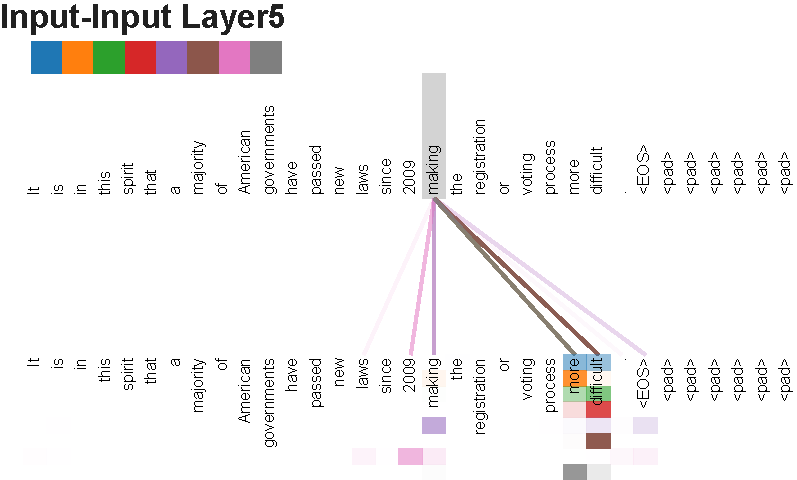
\includegraphics[width=\textwidth, trim=0 0 0 36, clip]{./vis/making_more_difficult5_new.pdf}}
\caption{一个展示编码器自注意力机制在6层中的第5层中处理长距离依赖关系的示例。许多注意力头关注动词`making'的远距离依赖,补全了短语`making...more difficult'。这里的注意力仅展示了单词`making'。不同颜色代表不同的注意力头。建议以彩色查看最佳效果。}
\end{figure*}

\begin{figure*}
{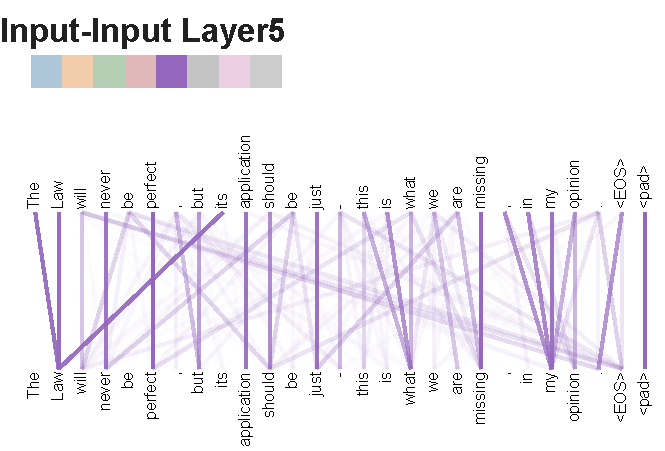
\includegraphics[width=\textwidth, trim=0 0 0 45, clip]{./vis/anaphora_resolution_new.pdf}}
{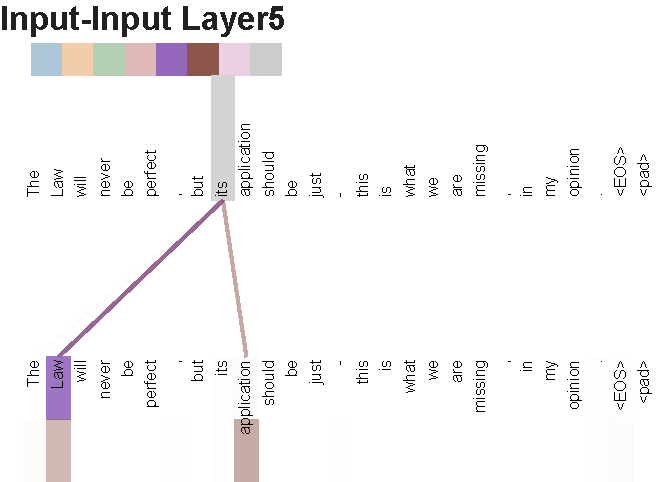
\includegraphics[width=\textwidth, trim=0 0 0 37, clip]{./vis/anaphora_resolution2_new.pdf}}
\caption{同样位于6层中的第5层的两个注意力头,显然参与了指代消解任务。上图:第5个注意力头的完整注意力分布。下图:仅针对单词`its'的第5和第6个注意力头的独立注意力分布。注意,对于这个词,注意力分布非常集中。}
\end{figure*}

\begin{figure*}
{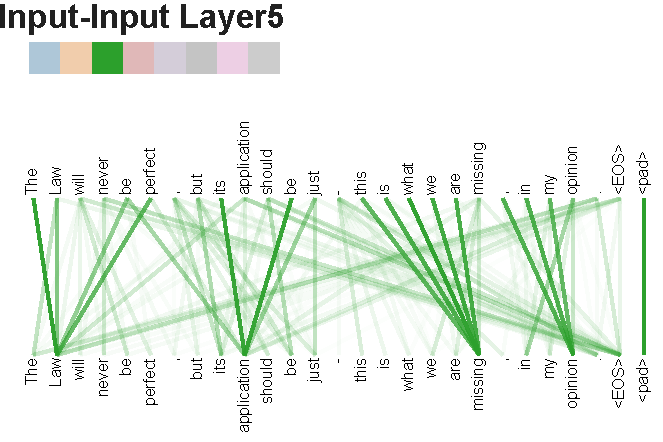
\includegraphics[width=\textwidth, trim=0 0 0 36, clip]{./vis/attending_to_head_new.pdf}}
{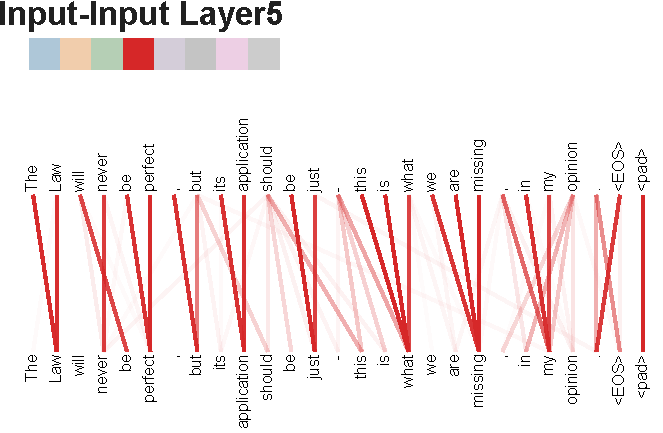
\includegraphics[width=\textwidth, trim=0 0 0 36, clip]{./vis/attending_to_head2_new.pdf}}
\caption{许多注意力头表现出的行为似乎与句子的结构有关。我们在上面给出了两个这样的示例,分别来自6层中第5层的编码器自注意力的两个不同注意力头。这些注意力头显然学会了执行不同的任务。}
\end{figure*}

\end{document}
